% demo.tex
%
% This file is part of the modernposter LaTeX template
%
% Version 1.03.1 2018/04/03
%
% Copyright 2018 David Derler and other contributors. A list of contributors 
% can be found at https://github.com/derlerd/modernposter/graphs/contributors
%
% This work is licensed under the Creative Commons Attribution-ShareAlike 4.0 
% International license (cf. https://creativecommons.org/licenses/by-sa/4.0/)  
% \documentclass[dvipdfmx]{modernposter}
%
% You may use the hlcolor option to pass a custom highlight color
% in HTML format. You may use the logo option to pass a path to
% a logo. You may use the helvet option to switch to the Helvetica
% font.
% 
\documentclass[a0paper,dvipdfmx,helvet,logo=logo.png,hlcolor=F70146]{modernposter}
\usepackage[T1]{fontenc}
\usepackage{lmodern}
\usepackage{tikz}
% \usepackage{gnuplot-lua-tikz}
\usepackage{empheq}
\usepackage{ulem}
\usepackage{amsmath, amsthm}
\usepackage{mathtools}
\usepackage{cases}
\usepackage{ascmac}
\usepackage{bbm}
\usepackage{ulem}
\usepackage{capt-of}
\usepackage{caption}
\usepackage{siunitx}
\usepackage{exscale}
\captionsetup[figure]{labelformat=empty}

\title{\fontsize{56pt}{1pt}\selectfont {A New Setting for Some Inverse Potential Problem and The Bubbling Method}}
\author{\fontsize{45pt}{1pt}\selectfont \underline{MORITA Ryuhei} \& IMAGAWA Masaki \& ISO Yuusuke} 
\email{Graduate School of Informatics, Kyoto University}

\begin{document}
\maketitle  

\begin{postercolumn}
  \posterbox{Abstract}{ 
    {\bf Can the potential take the place of the gravity?}

    We investigate the influence for reconstructing the shape of $\Omega$ 
    when we observe the potential or the gravity on $\partial B_a$.

    \begin{center}
      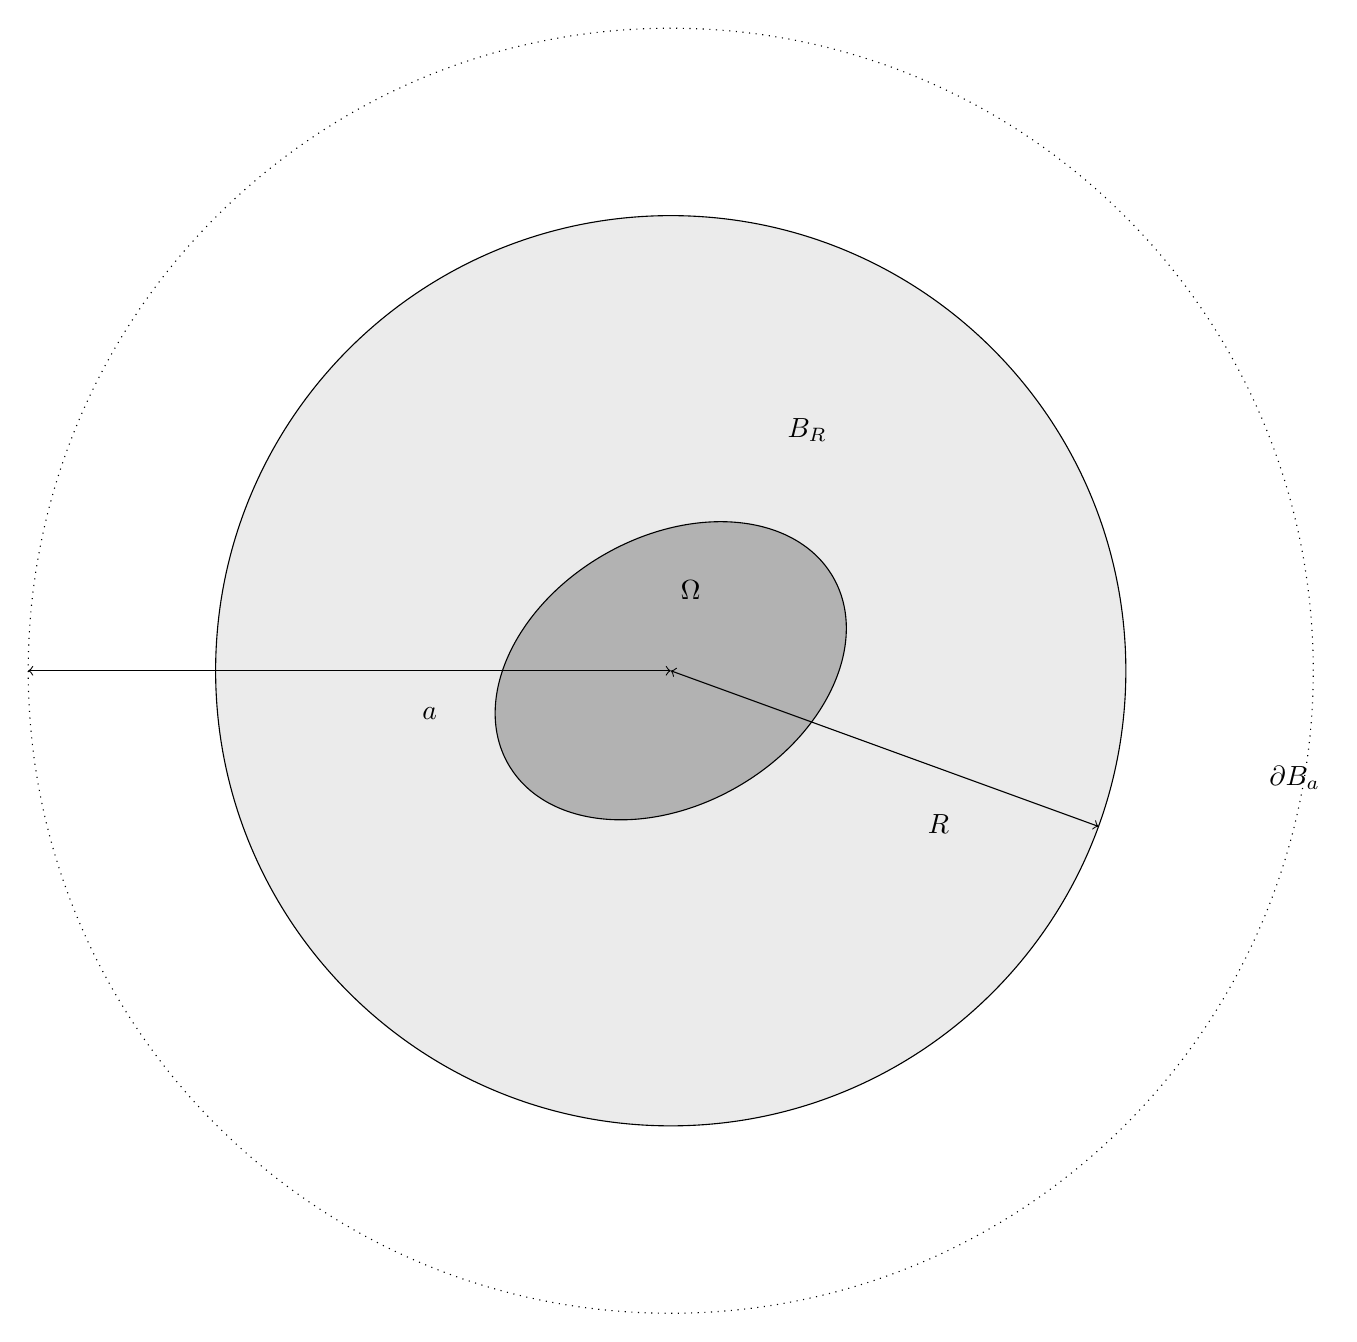
\begin{tikzpicture}[scale=3.4]
        \filldraw [fill=black!8!] (0,0)circle[radius=1.7];
        \filldraw [fill=black!30!] (-0,0)circle[x radius=0.7,y radius=0.5,rotate=30];
        \draw(0,0.3)node[right]{$\Omega$};
        \draw(0.4,0.9)node[right]{$B_R$};
        \draw(2.2,-0.4)node[right]{$\partial B_a$};
        \draw[<->](0,0)--({1.7*cos(-20)},{1.7*sin(-20)});
        \draw[<->](0,0)--(-2.4,0);
        \node[below] at (1,-0.5){$R$};
        \node[below] at (-0.9,-0.1){$a$};
        \draw[dotted] (0,0)circle[radius=2.4];
      \end{tikzpicture}
      \captionof{figure}{Core-Shell Body}
    \end{center}
  }

  \posterbox{Core-Shell Body}{
  The potential of Core-shell body $U$ is written as
  \begin{align*}
    U(x) = \underset{U^{B_R}}{\underline{\int_{B_R}E(x-y)dy}} + \rho\underset{U^{\Omega}}{\underline{\int_{\Omega}E(x-y)dy}},
  \end{align*}
  where $E$ is the Newton potential.

  The potential $\rho U^{\Omega}$ can be calculated on the $\partial B_a$.
  \begin{align*}
    \rho U^{\Omega} = U\text{(observed)} - U^{B_R}(\text{known})\quad \mathrm{on}\quad \partial B_a.
  \end{align*}

  % \begin{columns}
    % % \centering 
    % \begin{column}{0.48\textwidth}
      % % \centering
      % % \begin{tikzpicture}
        % % \filldraw [fill=black!10!] (0,0)circle[radius=1.0];
        % % \filldraw [fill=black!30!] (-0,0)circle[x radius=0.5,y radius=0.4,rotate=30];
        % % \draw(0,0)node{$\rho+1$};
        % % \draw(0,0.6)node{$\Omega$};
        % % % \draw[<->](0,0)--(-0.6,0);
        % % % \draw[<->](0,0)--({1.6*cos(-20)},{1.6*sin(-20)});
        % % \draw (0.4,-0.6)node{$1$};
        % % \draw (0,1.2)node{$B_R$};
        % % % \fill (0,0) circle (1pt); 
      % % \end{tikzpicture}
      % % \captionof{figure}{Core-shell body}
    % \end{column} 
    % % \hspace{-2cm}
    % % $\rightarrow$
    % % % \hspace{-1cm}
    \begin{center}
      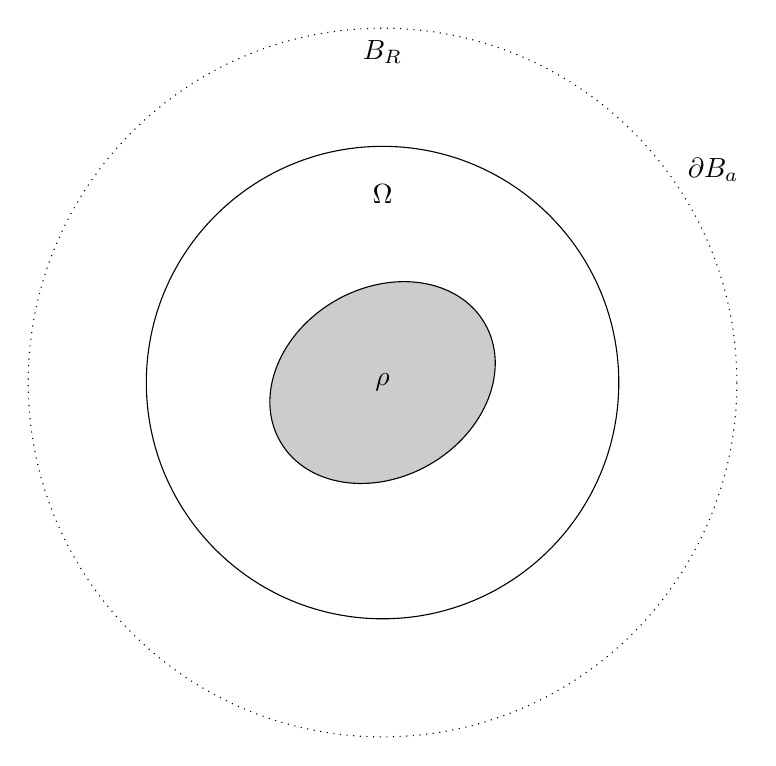
\begin{tikzpicture}[scale=3]
        \filldraw [fill=black!0!] (0,0)circle[radius=1.0];
        \filldraw [fill=black!20!] (-0,0)circle[x radius=0.5,y radius=0.4,rotate=30];
        \draw[dotted] (0,0)circle[radius=1.5];
        \draw(-0,0)node{$\rho$};
        \draw(0,0.8)node{$\Omega$};
        % \draw[<->](0,0)--(-0.6,0);
        % \draw[<->](0,0)--({1.6*cos(-20)},{1.6*sin(-20)});
        \draw (0,1.4)node{$B_R$};
        \draw (1.4,0.9)node{$\partial B_a$};
        % \fill (0,0) circle (1pt); 
      \end{tikzpicture}
      \captionof{figure}{Extract buried body}
    \end{center}

  % \end{columns}

  }

  \posterbox{Inverse Potential Problem} {
    \highlight{{\bf The potential observation has became possible by atomic clock!}}
    Observe the gravity or the potential on $\partial B_a$, and recover the shape of $\Omega$.
    
    \begin{center}
      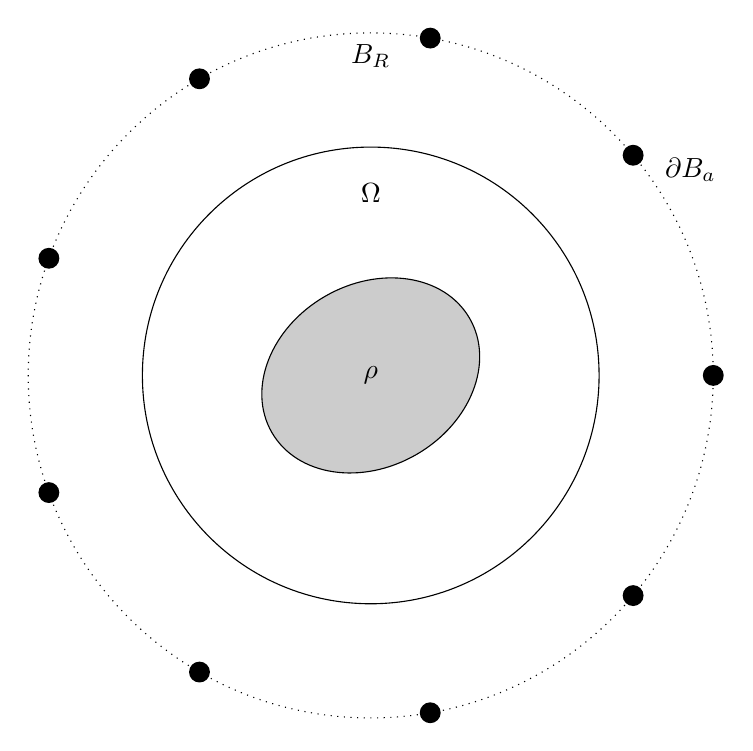
\begin{tikzpicture}[scale=2.9]
        \filldraw [fill=black!0!] (0,0)circle[radius=1.0];
        \filldraw [fill=black!20!] (-0,0)circle[x radius=0.5,y radius=0.4,rotate=30];
        \draw[dotted] (0,0)circle[radius=1.5];
        \draw(-0,0)node{$\rho$};
        \draw(0,0.8)node{$\Omega$};
        % \draw[<->](0,0)--(-0.6,0);
        % \draw[<->](0,0)--({1.6*cos(-20)},{1.6*sin(-20)});
        \draw (0,1.4)node{$B_R$};
        \draw (1.4,0.9)node{$\partial B_a$};
        % \fill (0,0) circle (1pt); 
        \fill ({1.5*cos(0)},{1.5*sin(0}) circle (1.3pt); 
        \fill ({1.5*cos(40)},{1.5*sin(40}) circle (1.3pt); 
        \fill ({1.5*cos(80)},{1.5*sin(80}) circle (1.3pt); 
        \fill ({1.5*cos(120)},{1.5*sin(120}) circle (1.3pt); 
        \fill ({1.5*cos(160)},{1.5*sin(160}) circle (1.3pt); 
        \fill ({1.5*cos(200)},{1.5*sin(200}) circle (1.3pt); 
        \fill ({1.5*cos(240)},{1.5*sin(240}) circle (1.3pt); 
        \fill ({1.5*cos(280)},{1.5*sin(280}) circle (1.3pt); 
        \fill ({1.5*cos(320)},{1.5*sin(320}) circle (1.3pt); 
      \end{tikzpicture}
    \end{center}

    % We can observe only at the finite points $\{A_n\}_{n=1}^N\subset\partial B_a$.
    \begin{itemize}
      \item Observation of Gravity (Traditional)
      \[
        \rho\nabla U^{\Omega} = \overrightarrow{g} \quad \mathrm{on} \quad \{A_n\}_{n=1}^N\subset \partial B_a
      \]
  
      \item \highlight{Observation of Potential (New)}
      \[
        \rho U^{\Omega} = p \quad \mathrm{on} \quad \{A_n\}_{n=1}^N\subset \partial B_a
      \]
    \end{itemize}

  }


\end{postercolumn} 

\begin{postercolumn}
  \doubleposterbox[0.5]{Sketch of Reconstruction Algorithm}{
    Reconstruction algorithm consists of two parts.
    \begin{enumerate}
      \item Approximate the body $\Omega$ by a set of point masses \\ → Optimization method
      \item Homogenize the set of point masses \\ → Bubbling method
    \end{enumerate}
  }
  {The Bubbling Method}{
  We homogenize the set of point masses to body with density $\rho$.
  \begin{center}
    \includegraphics[width=7cm]{fig3/move.png}
    \hspace{4cm}
    \includegraphics[width=6cm]{fig3/pms.png}
    % \begin{tikzpicture}
      % \draw [dotted,thin] (-1.25,-1.25) grid [step=1] (1.25,1.25);
      % \fill [red] (0,0) circle (3pt); 
      % \draw (0.35,0.40) circle (3pt); 
      % \fill (0.35,0.40) circle (2pt); 

      % \fill (1,0) circle (3pt);
      % \fill (1,1) circle (3pt);
      % \fill (0,1) circle (3pt);
      % \fill (-1,1) circle (3pt);
      % \fill (-1,0) circle (3pt);
      % \fill (-1,-1) circle (3pt);
      % \fill (0,-1) circle (3pt);
      % \fill (1,-1) circle (3pt);

      % \draw[<->](-1.3,-1)--(-1.3,0);
      % \node[left] at (-1.3,-0.5){$h$};

      % \draw(0.7,0.7)node{$M_{i,j}$};
      % \draw[->](0.25,0.30)--(0.1,0.1);
    % \end{tikzpicture}



    % \begin{tikzpicture}
      % \draw [dotted,thin] (-1.25,-1.25) grid [step=1] (1.25,1.25);
      % \fill [red] (0,0) circle (3pt); 
      % \fill [blue] (-1,0) circle (3pt); 
      % \fill [blue] (1,0) circle (3pt); 
      % \fill [blue] (0,1) circle (3pt); 
      % \fill [blue] (0,-1) circle (3pt); 

      % \fill (1,1) circle (3pt); 
      % \fill (1,-1) circle (3pt); 
      % \fill (-1,1) circle (3pt); 
      % \fill (-1,-1) circle (3pt); 

      % \draw(0.4,0.3)node{$\widetilde{M}_{i,j}$};
      % \draw[->](0.2,0)--(0.5,0);
      % \draw[->](0,0.2)--(0,0.5);
      % \draw[->](-0.2,0)--(-0.5,0);
      % \draw[->](0,-0.2)--(0,-0.5);
    % \end{tikzpicture}
  \end{center}

  }

  \posterbox{Reconstruction of Ellipzoid}{
    \begin{center}
      \includegraphics[width=9cm]{fig/elliptic.png}
      \captionof{figure}{Source}
    \end{center}

    \begin{itemize}
      \item Observation of Gravity ($a=10, 30, 200$)
      \begin{center}
        \includegraphics[width=9cm]{fig2/GN300K100R10E2.png}
        \includegraphics[width=9cm]{fig2/GN300K100R30E2.png}
        \includegraphics[width=9cm]{fig3/GN300K100R200E2.png}
      \end{center}

      \item \highlight{Observation of Potential} ($a=10, 30, 200$)
      \begin{center}
        \includegraphics[width=9cm]{fig2/PN300K100R10E2.png}
        \includegraphics[width=9cm]{fig2/PN300K100R30E2.png}
        \includegraphics[width=9cm]{fig3/PN300K100R200E2.png}
      \end{center}
    \end{itemize}
  }

  \posterbox{Conclusion}{
    We observe the potential and reconstruct the shape of the body, compared to observation of the gravity.

    \begin{itemize}
      \item Reconstruction of Ellipzoid

      In this case, reconstruction by observation of the potential can reconstruct source body more correctly.

    \end{itemize}

    \begin{center}
      \centering
      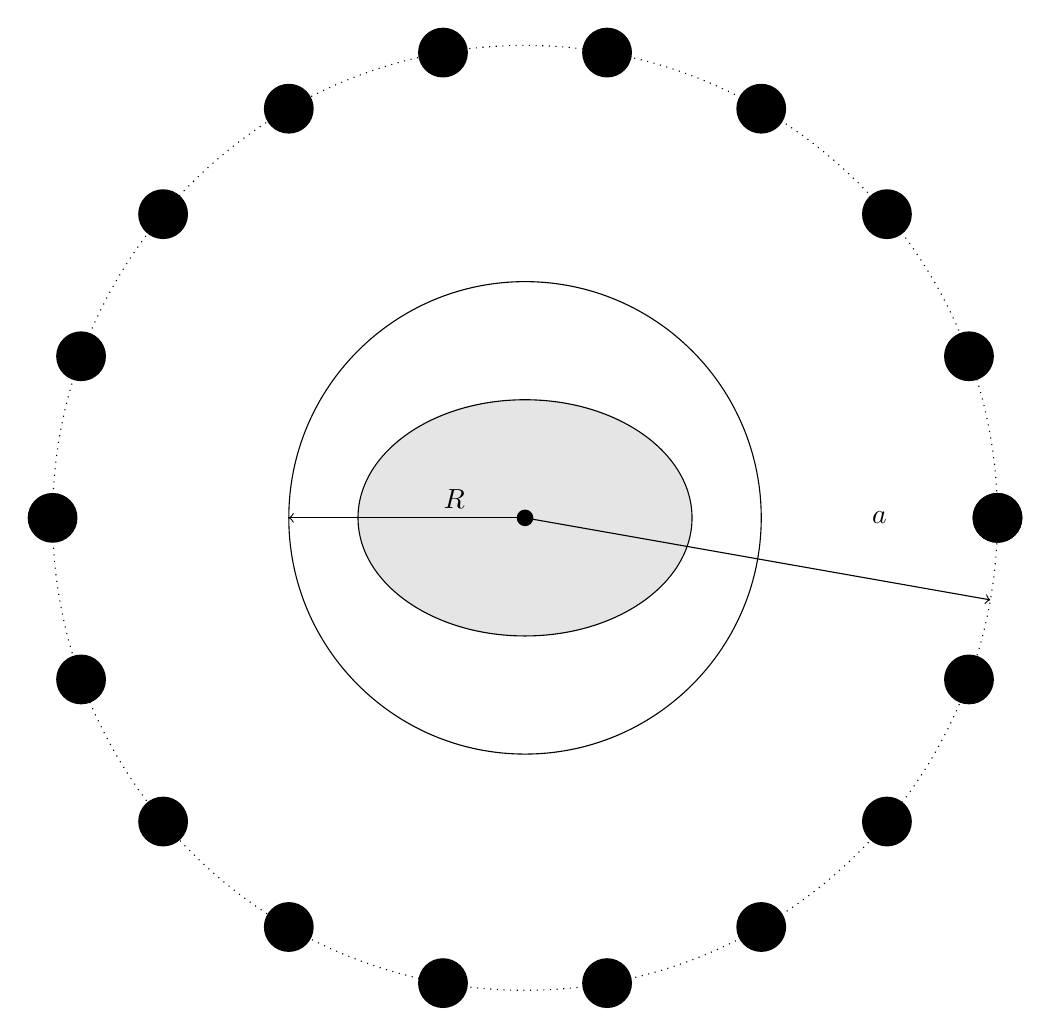
\begin{tikzpicture}[scale=3]
        % \filldraw[fill=black!10!] ({-0.25*sqrt(3)},-0.25) -- ++(0:{0.5*sqrt(3)}) -- ++(120:{0.5*sqrt(3)}) -- cycle;
        \filldraw [fill=black!10!] (0,0)circle[x radius=0.707,y radius=0.5,rotate=0];
        \fill (0,0) circle (1pt); 
        \draw (0,0)circle[radius=1];
        \draw[<->](0,0)--(-1,0);
        \draw[<->](0,0)--({2*cos(-10)},{2*sin(-10)});
        \draw(1.5,0)node{$a$};
        \draw(-0.3,0)node[above]{$R$};
        \draw[dotted] (0,0)circle[radius=2];
        \fill (2,0) circle (3pt); 
        \fill ({2*cos(0)},{2*sin(0}) circle (3pt); 
        \fill ({2*cos(20)},{2*sin(20}) circle (3pt); 
        \fill ({2*cos(40)},{2*sin(40}) circle (3pt); 
        \fill ({2*cos(60)},{2*sin(60}) circle (3pt); 
        \fill ({2*cos(80)},{2*sin(80}) circle (3pt); 
        \fill ({2*cos(100)},{2*sin(100}) circle (3pt); 
        \fill ({2*cos(120)},{2*sin(120}) circle (3pt); 
        \fill ({2*cos(140)},{2*sin(140}) circle (3pt); 
        \fill ({2*cos(160)},{2*sin(160}) circle (3pt); 
        \fill ({2*cos(180)},{2*sin(180}) circle (3pt); 
        \fill ({2*cos(200)},{2*sin(200}) circle (3pt); 
        \fill ({2*cos(220)},{2*sin(220}) circle (3pt); 
        \fill ({2*cos(240)},{2*sin(240}) circle (3pt); 
        \fill ({2*cos(260)},{2*sin(260}) circle (3pt); 
        \fill ({2*cos(280)},{2*sin(280}) circle (3pt); 
        \fill ({2*cos(300)},{2*sin(300}) circle (3pt); 
        \fill ({2*cos(320)},{2*sin(320}) circle (3pt); 
        \fill ({2*cos(340)},{2*sin(340}) circle (3pt); 
      \end{tikzpicture}
    \end{center}

  }
\end{postercolumn}
 
\end{document}